\section{Imperative to Streaming Transformation}
\label{sec:control}

%In a na\"ive approach, we can map each controller in the hierarchy into a VB (\Cref{fig:centralctrl}).
%This strategy suffers from expensive network round-trip delays between the parent and child controllers.
%If the parent controller is an unrolled loop, the parent needs to synchronize with all child controllers, which creates an undesired communication hot spot.
%\Cref{fig:centralctrl}(a) shows an example where synchronization {\em just} between parent and child controllers can produce an incorrect result due to unpredictable network latency.

%The alternative approach explores a different way to execute the expected control schedule correctly. 
%The minimum required synchronization to produce the correct result is to ensure that the computations access the intermediate results in a consistent matter as if the control schedule is strictly enforced. 
%This can be achieved via p2p synchronizations \emph{only} between computations that access a particular shared memory.
%The execution order of computations that access different memories does not need to be enforced, as they do not impact the program outcome.
%Therefore, as long as the compututation is executed with the expected number of iterations and the memories are updated consistently, there is no need for any extra synchronization.
%Next, we walk through how \name{} achieves this in more concrete detail.

\subsection{Loop Division}
Reviewing the front-end and back-end abstraction of \name, an obvious gap between the two
abstractions is that the front-end imperative language can contain arbitrary nested control hierarchy, whereas
the hardware compute engine can only execute perfectly nested loops.
To address this issue, we introduce a new type of loop transformation---loop division---for streaming reconfigurable
accelerators.
Similar to loop fission, loop division breaks a single loop into multiple loops.
The difference is that loop fission generates a sequence of sequentially executed loops, whereas
loop division generates loops executing \emph{concurrently}.
Additionally, loop fission materializes the intermediate results across fissioned loops into arrays,
while loop division use queue to communicate across loops.
Each loop generated from loop division can only execute if all of their input queues is not empty.
\Cref{fig:loopexp1} gives an example of loop fusion vs. loop division.

\begin{figure*}
\centering
\begin{subfigure}[b]{0.28\textwidth}
\inputminted{python}{code/loopexp1.py}
\caption{Input program}
\end{subfigure}
\hfill
\begin{subfigure}[b]{0.31\textwidth}
\inputminted{python}{code/loopexp1fission.py}
\caption{Loop Fission}
\end{subfigure}
\hfill
\begin{subfigure}[b]{0.32\textwidth}
\inputminted{python}{code/loopexp1division.py}
\caption{Loop Division}
\end{subfigure}
\caption[Example of Loop Fission vs. Loop Division]{
  (b) and (c) shows the output of loop fission and loop division of the input program (a), respectively.
  In (b), the first loop is executed entirely before executing the second loop. The intermediate
  result \texttt{tmp} is materialized into an array with the same size as the loop range.
  In (b), the two loops can execute concurrently. The intermediate result is materialized into a
  queue. For each iteration, a loop can execute only if all of its queues are non-empty.
  The second loop can execute as soon as \texttt{tmp} receives the first element.
}
\label{fig:loopexp1}
\end{figure*}

When executing loop division on a single-threaded CPU, the CPU must context switching between the
concurrent loops
and executing the one with cleared input dependencies.
Like loop fission, loop division is likely worsen the performance on a processor architecture, as
the memory footprint of the intermediate result \texttt{tmp} increases from $O(1)$ to $O(N)$.
On RDAs, the devisied loops are executing
concurrently in streaming pipelined fashion. The size of the \texttt{tmp} can be limit to a small fixed
size, efficiently implemented with a hardware FIFO. 
Although loop transformations are generally optimizations on CPUs,
loop division is a required transformation to converts an infeasible program to a feasible one for Plasticine.

Loop fission is not always safe, as it may alters the execution order of the program.
order.
Loop division, on the other hand, does not change the underlying data-dependency and is always safe.
To achieve this, loop division needs to introduce additional dummy data dependency to enforce the correct 
execution.
\Cref{fig:loopexp2} gives an example of an invalid loop fission and a correct loop division.
\Cref{fig:sync} gives more detail on how the dummy data-dependency are generated automatically.

\begin{figure*}
\centering
\begin{subfigure}[b]{0.28\textwidth}
\inputminted{python}{code/loopexp2.py}
\caption{Input program}
\end{subfigure}
\hfill
\begin{subfigure}[b]{0.32\textwidth}
\inputminted{python}{code/loopexp2fission.py}
\caption{Invalid Loop Fission}
\end{subfigure}
\hfill
\begin{subfigure}[b]{0.31\textwidth}
\inputminted{python}{code/loopexp2division.py}
\caption{Loop Division}
\end{subfigure}
\caption[Example of Loop Fission vs. Loop Division]{
Example of Loop Fission vs. Loop Division
}
\label{fig:loopexp2}
\end{figure*}

\subsection{Virtual Context Allocation} 

\begin{figure*}
\centering
\begin{subfigure}[b]{0.4\textwidth}
\inputminted{python}{code/spatialeg.py}
\caption{Pseudo input example}
\label{fig:contexteg}
\inputminted{python}{code/contextalloc.py}
%\missingfigure[figwidth=1\textwidth]{Spatial IR}
\caption{Context allocation}
\end{subfigure}
\hfill
\begin{subfigure}[b]{0.5\textwidth}
\inputminted{python}{code/contextsplit.py}
\caption{Request and response division}
\end{subfigure} \\
\vspace{0.2cm}
\begin{subfigure}[b]{0.23\textwidth}
%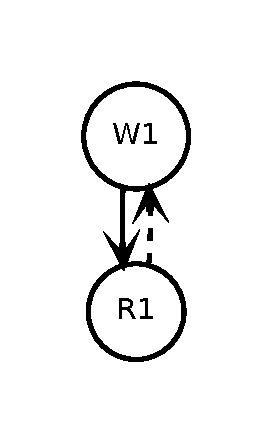
\includegraphics[width=1\textwidth]{figs/dep.pdf}
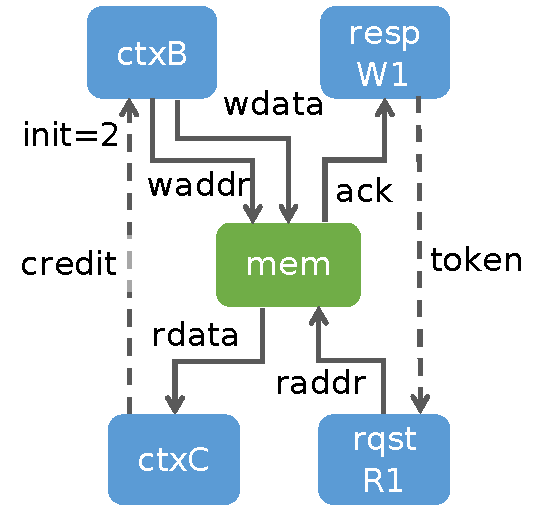
\includegraphics[width=1\textwidth]{figs/ctxdag.pdf}
\caption{Context Graph}
\end{subfigure}
\begin{subfigure}[b]{0.76\textwidth}
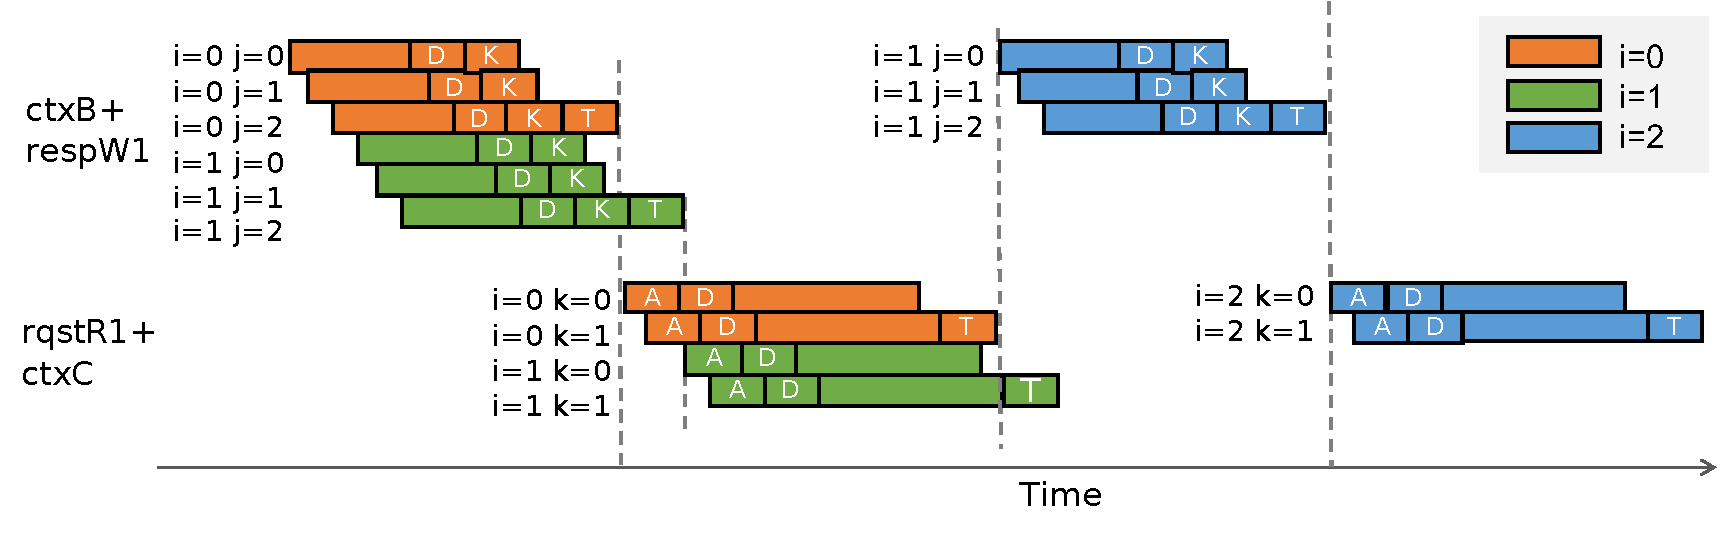
\includegraphics[width=1\textwidth]{figs/plasticinetiming.pdf}
\caption{Timing on Plasticine}
\end{subfigure}
\caption[Context allocation]{
  Lowering example.
  %Same example as \Cref{fig:spatialegpar} without outer loop
  %unrolling factor equals to 1.
  %(a) has two basic blocks within the inner most controllers \texttt{B} and \texttt{C}.
  \name allocates one context per basic block for \texttt{B} and \texttt{C}, shown in (b). Outer controller \texttt{A} is
  duplicated in both \texttt{ctxB} and \texttt{ctxC}.
  (c) \name seperates out requestion generator \texttt{rqstR1} from \texttt{ctxB} for \texttt{R1} 
  and response receiver from \texttt{ctxC} \texttt{respW1} for \texttt{W1}.
  The resulting dataflow graph is shown in (d). 
  To enforce the forward data-dependency between \texttt{W1} and \texttt{R1}, 
  \name allocates a forward token between \texttt{W1}'s response receiver \texttt{respW1} and
  \texttt{R1}'s request generator \texttt{rqstR1};
  to enforce the loop-carried WAR dependency between \texttt{R1} and \texttt{W1}, \name allocates a
  backward token (\texttt{credit}) between \texttt{R1}'s response receiver \texttt{ctxC} and 
  \texttt{W1}'s request generator \texttt{ctxB}. 
  The backward credit is initialized with two elements because \texttt{mem} is double-buffered.
  On the writer side, a forward \texttt{token} is a
  produced and a backward \texttt{credit} is consumed every \texttt{B} iterations; on the reader
  side, a forward \texttt{token} is consumed and a backward credit is produced every \texttt{C}
  iterations. The resulting timing of the execution is shown in (e).
}
\label{fig:contextalloc}
\end{figure*}

As a start, \name allocates one virtual memory to hold each on-chip data structure, and 
one context to execute each basic block within the inner most controllers. 
A basic block maps naturally to a context, as instructions within a basic block are control-free. 
Next, \name makes a copy of all controllers enclosing the basic block in the corresponding context;
these controllers are later converted to counters and control configurations supported by the
hardware. 
\Cref{fig:contextalloc} shows an example of the context allocation. 
With these controllers, contexts can repeat execution for expected number iterations. However,
data-structures written and read by different contexts are accessed in random order.
The insight is that \emph{as long as all contexts accessing a shared memory with expected program order,
the final result is identical to a sequentially executed program}.
Unlike traditional out-of-order execution, where hardware and compiler look for independent instructions to
execute concurrently, \name starts with executing \emph{all} basic blocks in a program in \emph{concurrent} contexts.
Next, \name introduces synchronizations to maintain consistent access order as expected by the 
program \emph{only} among contexts accessing a shared memory. 
This way, \name introduces minimum p2p synchronizations among small groups of contexts; contexts
accessing different memories are naturally parallelized without impacting the final output.

\subsection{Control Allocation} 
\label{sec:sync}
Starting with all contexts execute in parallel, \name introduces \term{control token}s across contexts
to serialize their execution order based on the program order.
This control token is no different from a regular data-dependency and can be viewed as 
an access grant to the shared memory across contexts. 
By controlling {\em where}, {\em how}, and {\em when} to pass the token, \name 
is able to maintain a consistent update ordering between the pipelined and parallelized contexts that 
access the shared memory.

We refer to an memory access appeared in the input IR as a \emph{declared access}, as supposed to
memory accesses executed at runtime.
\texttt{W1} and \texttt{R1} are examples of two declared accesses in \Cref{fig:contexteg}
In the rest of this section, we will walk through the detail on how \name allocates control tokens
to maintain sequential consistency on Plasticine.

\begin{table*}
  \centering
\begin{tabular}{lccc}
  \toprule
 Data structure & Memory type \\ \midrule
  array (fit on-chip) & SRAM \\
  array (not fit on-chip) & DRAM \\
  scalar variable & register \\
  queue & FIFO \\
 \bottomrule
\end{tabular}
\caption[Mapping between data-structure to hardware memories]{
  Mapping between user declared data-structure to underlying hardware memories. 
  Programmers explicitly specify the desired hardware type inside Spatial. 
  In other languages, this table specifies a mapping between software data-structures 
  and hardware memory types on Plasticine.
}
\label{tab:memtype}
\end{table*}

\paragraph{Where.}
During control allocation, \name examines all declared accesses of a memory and checks for dependency across these accesses.
\name only allocate resource to synchronize two contexts if they contain declared accesses that can potentially interfere.
Whether two declared accesses interfere depends on 
\begin{outline}
  \1 the type of accesses (read vs. write)
  \1 the type of the memory (e.g. SRAM, DRAM)
  \1 and location of the declared accesses in the control hierarchy.
\end{outline}

\begin{table*}
  \centering
\begin{tabular}{lcccc}
  \toprule
  Memory type             & DRAM   & SRAM   & FIFO   & Register \\ \midrule
  read-after-read (RAR)   & \xmark & \cmark & \cmark & \cmark \\
  read-after-write (RAW)  & \cmark & \cmark & \cmark & \cmark \\
  write-after-read (WAR)  & \cmark & \cmark & \cmark & \cmark \\
  write-after-write (WAW) & \cmark & \cmark & \cmark & \cmark \\
 \bottomrule
\end{tabular}
\caption[Interferance Table]{
  Interference table for whether two accesses interfere for each memory type.
}
\label{tab:interferetab}
\end{table*}

\Cref{tab:memtype} lists hardware memories available on reconfigurable architectures and software
data-structures providing similar program semantics.
The type of the memory matters because they have different programming interface in the hardware.
For instance, two read accesses does not interfere for DRAM because the DRAM interface permits
multiple concurrent access streams through multiple DAGs\footnote{All DAGs can access the full DRAM
address space}. 
\gist{mension port virtualization}
Therefore, from the programmer perspective, users do not need
to serialize the two contexts reading the same DRAM address. 
SRAMs, on the other hand, have single read 
and write ports. Programmers must guarantee that a PMU receives read requests from a single context
at any point in time for correctness.
\Cref{tab:interferetab} shows the interference relation between different types of memory across
accesses.

\begin{figure*}
\centering

\begin{subfigure}[b]{0.5\textwidth}
\begin{figure*}
\centering
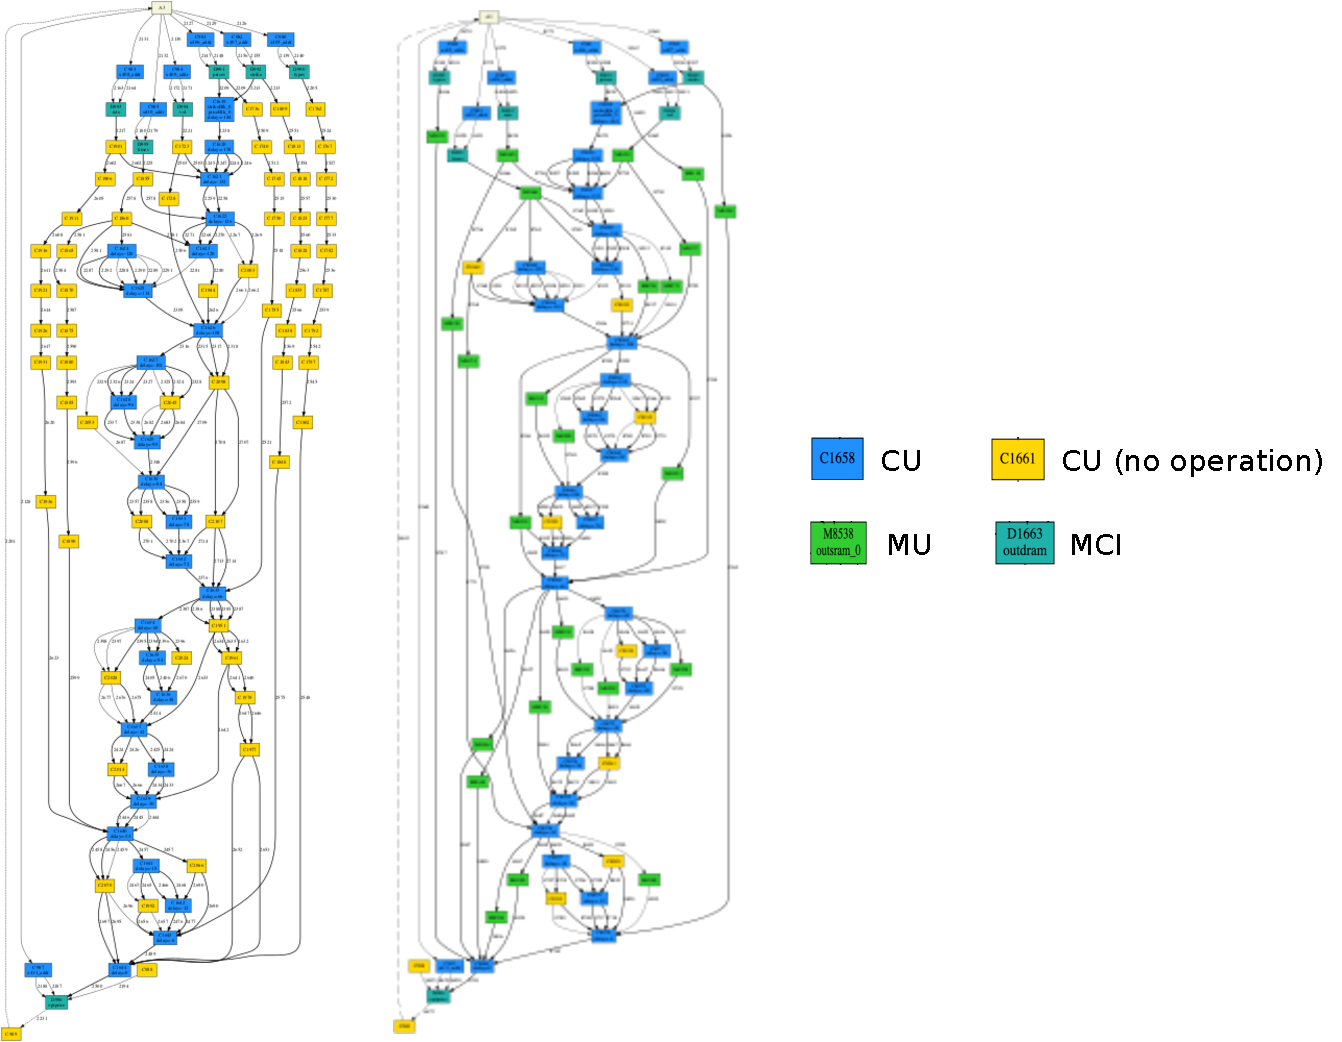
\includegraphics[width=0.7\textwidth]{figs/retiming.pdf}
\caption[Retiming]{
  Left: retiming with input buffer only. Right: retiming with either input buffer or scratchpad.
}
\label{fig:mlp}
\end{figure*}
\inputminted{python}{code/dep1.py}
\caption{Pseudo example}
\end{subfigure}
\begin{subfigure}[b]{0.3\textwidth}
  \centering
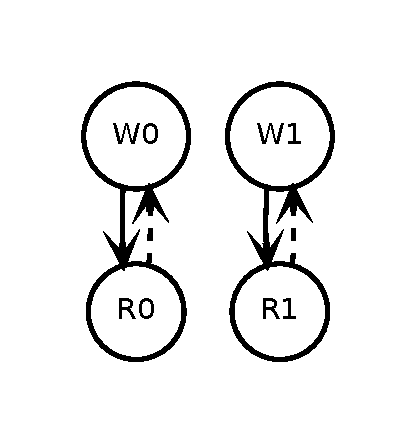
\includegraphics[width=0.8\textwidth]{figs/dep1.pdf}
\caption{Dependency Graph}
\end{subfigure}
\\
\begin{subfigure}[b]{0.5\textwidth}
\inputminted{python}{code/dep3.py}
\caption{Pseudo example}
\end{subfigure}
\begin{subfigure}[b]{0.3\textwidth}
  \centering
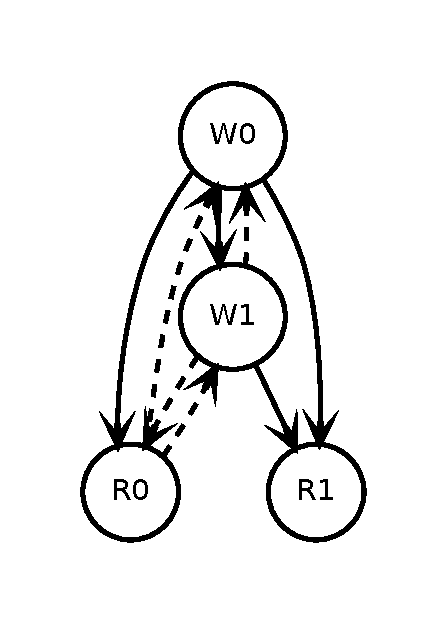
\includegraphics[width=0.8\textwidth]{figs/dep3.pdf}
\caption{Dependency Graph}
\end{subfigure}

\caption[Dep Graph]{
    Dep Graph
}
\label{fig:depexp}
\end{figure*}

For every declared access, \name{} checks on other accesses appeared earlier in the program order
for a possible forward dependency, and later in the program order for a possible loop-carried dependency (LCD). 
In the example in \Cref{fig:contexteg}, there is a forward data dependency between \texttt{W1} and
\texttt{R1}, and a LCD between \texttt{R1} and \texttt{W1}. 
\name builds a dependency graph between declared accesses for each memory.
\Cref{fig:depexp} gives more examples on how \name
determines dependencies based on where these accesses are declared in the control hierarchy.

Enforcing all dependencies in the dependency graph may not be necessary, as enforcing a subset of
dependencies can be sufficient to enforce the order of the whole graph.
Therefore, \name performs a transitive reduction (TR) on the graph to keep the minimum number of dependency edges 
that preserve the same ordering \cite{tr}.
Since TR on a cyclic graph is NP-hard, ]name perform TRs on the forward and backward LCD graphs, separately.
Notice, dependencies between accesses touching different buffers of a multi-buffered memory is less rigid 
than accesses touching the same buffer.
Therefore, we can only remove an edge if all dependencies on the equivalent path have a stronger or equivalent 
dependency strength than the strength of the removed edge.

%Two declared accesses A and B have no dependency if their least-common ancestor (LCA) controller executes only one of the children at anytime (from a branch), or all children in parallel (from an unrolled loop).
%The LCD exists between B to A, if B occurs later in the program order, and A and B are surrounded by a loop.
%To detect LCD, \name checks if a loop exists among two accesses' LCA controller and LCA's ancestor controllers.

\begin{figure*}
\centering
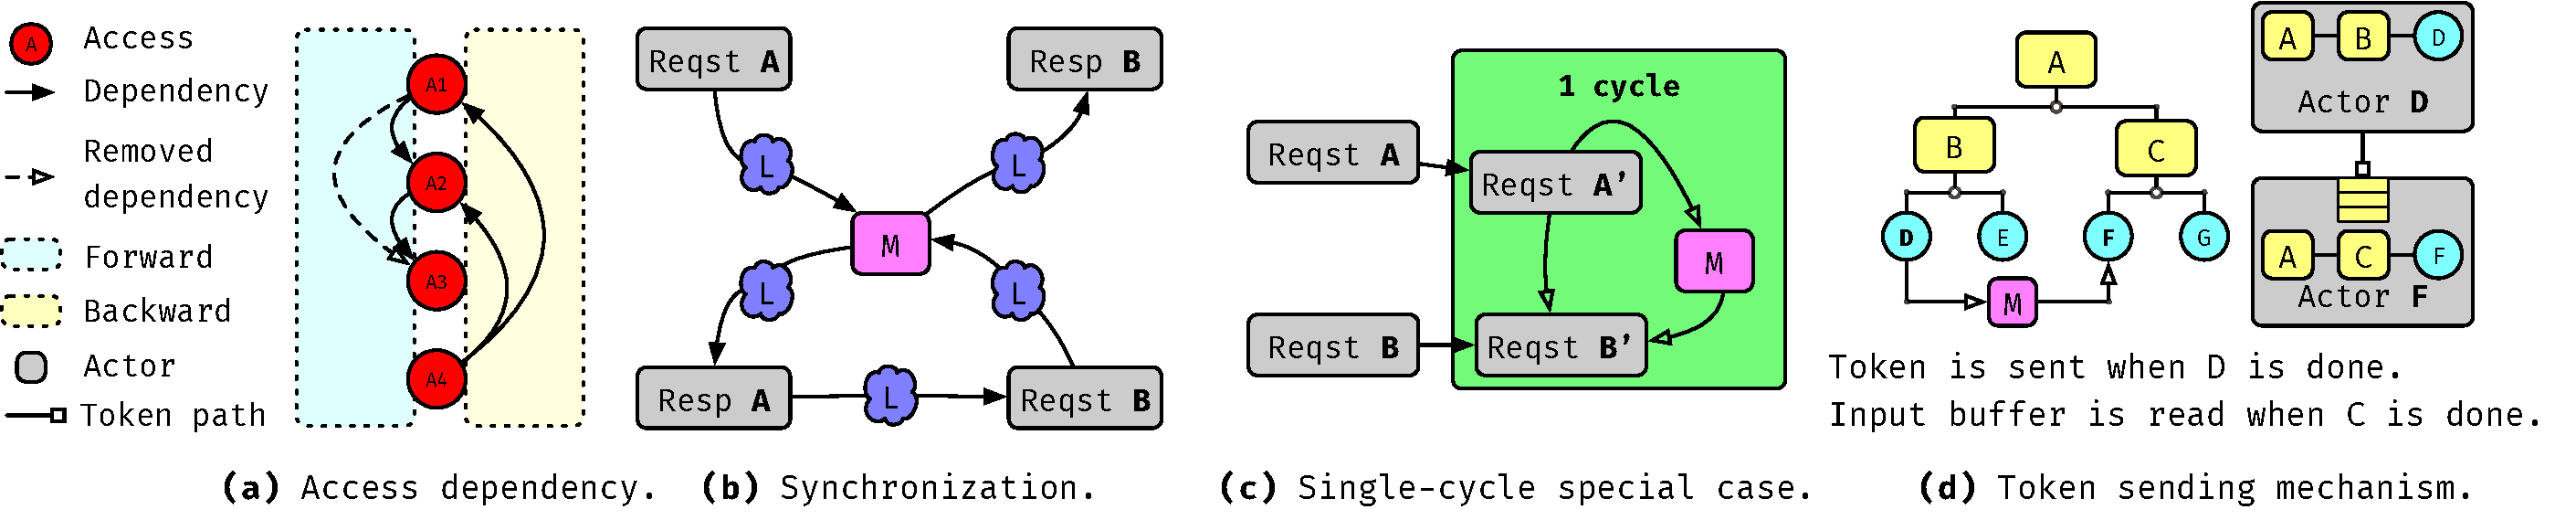
\includegraphics[width=1.0\textwidth]{figs/synch_mech.pdf}
\caption{
    (a) Access dependency graph.
    (b) Synchronization of two accesses on the same memory.
    (c) Single-cycle special case.
    (d) Actors uses local states of controller hierarchy to determine when to send a token.
}\label{fig:depgraph}\label{fig:token}\label{fig:tokentrick}\label{fig:tokenwhen}
\end{figure*}
%\ms{repeated caption, rather give a single caption.}

\paragraph{How.} 
%For each intermediate memory, \name{} builds a dependency graph for all its declared accesses (\Cref{fig:depgraph}(a)).
%Enforcing all dependencies in this graph may not be necessary as dependencies between $A_1$ and $A_2$, and $A_2$ and $A_3$ already capture the dependency between $A_1$ and $A_3$.

To eliminate the round-trip overhead between the memory and the computation, 
\name{} duplicates the local states and expressions required to generate the requests in a separate actor as the one that handles the responses.
For write accesses, the memory provides an acknowledgment for each request received, used by \name for synchronization.
The request actor generates requests asynchronously as soon as its data-dependencies are cleared, pushing all requests to memory until back-pressured.
To order a declared access A before a declared access B
\name creates a dummy dependency between the actor that accumulates the response of access A ($resp_A$) and the actor that generates requests for access B ($reqst_B$) (\Cref{fig:token}(b)).
To enforce LCD from access B to access A, \name introduces a token from $resp_B$ to $reqst_A$, and initializes the token buffer (input buffer receiving the token) with one element to enable the execution of the first iteration.
If the LCD is on a multi-buffered memory, the LCD token is initialized with the buffer depth number of elements to enable A for multiple iterations before blocked by access B.

These are general schemes we use on any types of memory (including DRAM and on-chip memories) with unpredictable access latency.

\subparagraph{Special Case: Single-Cycle Access}
For a memory with guaranteed {\em single-cycle} access latency, such as registers and statically banked SRAMs that are guaranteed conflict-free, we can simplify the necessary synchronization (\Cref{fig:tokentrick}(c)).
Instead of synchronizing between $resp_A$ and $reqst_B$, we allocate two stateless actors $reqst_A'$ and $reqst_B'$ within {\emph the same} VB as the accessed memory that forwards requests from $reqst_A$ and $reqst_B$, respectively.
Next, we forward the token going from $reqst_A$ to $reqst_B$ to go through $reqst_A'$ to $reqst_B'$ instead, and configure the token buffer in $reqst_B'$ with the depth of one for serialized schedule and depth of M for multi-buffered schedule. 
We no longer need to insert the LCD token, as the stiff back pressure from the token buffer in $reqst_B'$ will enforce the expected behavior.
This optimization only works if the sender and receiver of the token buffer are physically in a single VB where the memory is located.
In this way, when $reqst_B'$ observes $reqst_A'$s token, $reqst_B'$ is guaranteed to observe the memory update from $reqst_A'$ because the memory also has single-cycle access latency.

\paragraph{When.}
\name{} configures the actors to generate the token using their local states at runtime.
For FIFOs, the token is generated and consumed every cycle when the producer and receiver actors are active.
For register, SRAM, and DRAM the program order expects that the producer and consumer writes and inspects the memory once per iteration of their LCA controller, respectively.
Since the producer and receiver both have their outer controllers duplicated in their local state, they have independent views for one iteration of the LCA controller, which is when the controller in their ancestors (that is the immediate child of the LCA controller) is completed (\Cref{fig:tokenwhen}(d)).
The {\em done} signals of these controllers are used to produce and consume the token in actors, independently.

\subsection{Data-Dependent Control Flow}
Using the synchronization discussed in \Cref{sec:sync}, we can support control constructs that typically are not supported on most RDAs, such as branch and a while convergence loop.
The controllers in the input graph can also have data dependencies, such as loop ranges. 
The dynamic-loop ranges are handled as data dependencies to actors with \emph{memory localization} described in \Cref{sec:sync}.
The branch condition is also treated as a data-dependent enable signal of controllers under branch clauses.
If the controller is disabled, it is considered {\em done} immediately.
Output tokens depending on the {\em done} signal will be immediately sent out.
For a memory written inside a branch statement and read outside the branch (with a branch miss), the writer actor immediately sends out the token to the receiver
as soon as the branch condition is resolved. 
With a branch hit, the controller waits until its inner controller completes before raising the {\em done} signal.
%This way, the 
A similar scheme is used to implement the while loop, where the while condition is a data-dependency of stop signal of controller X. 
The producer of the while condition also consumes its own output as an LCD. 
The condition is then broadcast to all other actors under the same while loop. 
The {\em done} signal of the while loop is raised when the condition's data-dependency evaluates to true.
At this point, actors accessing memory within the while loop will send the token to access actors outside of the while loop, and enable them to access the intermediate memory.

After all actors and shared resources are allocated and synchronized, we simply put each actor and shared resource into their own VBs.
The actors with single-cycle special case (\Cref{sec:sync}) must be put in the same VB as the shared memory.

